\documentclass[12pt,a4paper]{report}
\usepackage[T2A]{fontenc}
\usepackage[utf8]{inputenc}
\usepackage[russian]{babel}
\usepackage{graphicx, setspace}

\usepackage[
top = 1.25cm, 
bottom = 2.0cm]{geometry}

\begin{document}
\begin{titlepage} 
	\centering
    % HEADER
	{
        \scshape
        Федеральное государственное автономное образовательное учреждение высшего образования
        \par
        \textbf{«Научно-образовательная корпорация ИТМО»}
        \par
        \vspace*{1cm}
        Факультет Программной Инженерии и Компьютерной Техники
        \par
    }
    % LOGO
    \vspace*{0.6cm}
    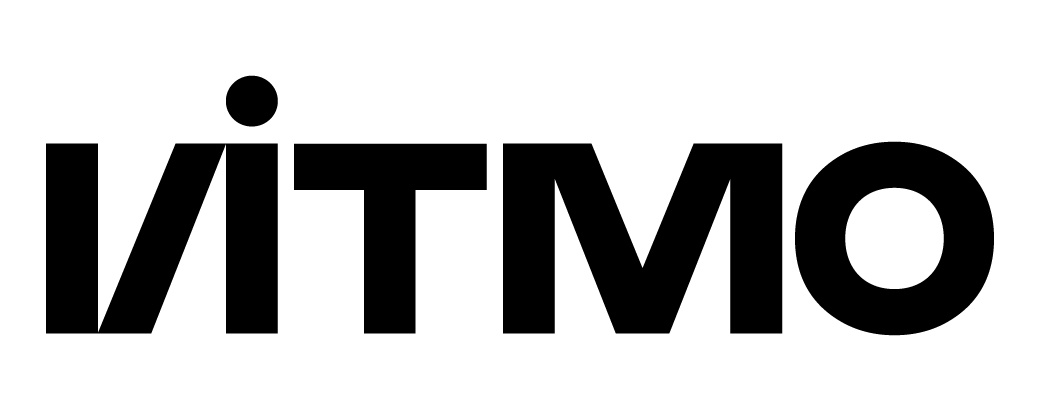
\includegraphics[width=\textwidth]{logo.png}
    % LAB INFO
    {
        \Large
        \textbf{Лабораторная работа по ОПД №5}
        \par
        \normalsize
        \vspace*{0.75cm}
        \textbf{Вариант 957}
        \par
    }
    \vfill
    % СREDITS
    \hfill\begin{minipage}{\dimexpr\textwidth-7.8cm}
        \textbf{Выполнил:}\par
        Степанов Арсений Алексеевич\par
        \vspace*{0.15cm}
        \textbf{Группа:}\par
        P3109\par
        \vspace*{0.15cm}
        \textbf{Преподаватель:}\par
        Ткешелашвили Нино Мерабиевна\par
    \end{minipage}
    \vfill
    Санкт-Петербург, \the\year{}г.
\end{titlepage}  
\section*{Задание}
По выданному преподавателем варианту разработать программу асинхронного обмена данными с внешним устройством. При помощи программы осуществить ввод или вывод информации, используя в качестве подтверждения данных сигнал (кнопку) готовности ВУ.
\begin{itemize}
    \item Программа осуществляет асинхронный вывод данных на ВУ-1
    \item Программа начинается с адреса 0C6. Размещаемая строка находится по адресу 58A
    \item Строка должна быть представлена в кодировке КОИ-8
    \item Формат представления строки в памяти: АДР1: СИМВ1 СИМВ2 АДР2: СИМВ3 СИМВ4 ... СТОП\_СИМВ
    \item Ввод или вывод строки должен быть завершен по символу c кодом 0D (CR). Стоп символ является обычным символом строки и подчиняется тем же правилам расположения в памяти, что и другие символы строки.
\end{itemize}
\section*{Вывод}
Я научился работать с ассемблером в базовой ЭВМ, а также осуществлять асинхронный обмен данными с уcтройствами ввода/вывода
\end{document}